
\subsection{Arquitectura y funcionamiento de las Redes Neuronales Convolucionales}
\label{sec:cnn_fundamentos}

Las Redes Neuronales Convolucionales (CNN) son arquitecturas de aprendizaje profundo especializadas en el procesamiento de datos enfocados a imágenes y videos. Su funcionamiento se basa en la extracción de representaciones visuales de complejidad creciente; las primeras capas identifican características básicas como bordes, mientras que las capas subsecuentes reconocen texturas, partes y, finalmente, objetos completos \cite{goodfellow2016deep}.

Sus aplicaciones principales abarcan la clasificación de imágenes, la detección de objetos, la segmentación semántica y el reconocimiento facial, consolidándose como el estándar en tareas de visión por computadora. Desde una perspectiva histórica, la arquitectura LeNet-5 (LeCun, 1989) sentó las bases para el reconocimiento de dígitos escritos a mano. Posteriormente, la arquitectura AlexNet detonó el auge del aprendizaje profundo moderno al ganar la competencia ImageNet, reduciendo el error top-5 de aproximadamente 26\% a 15\% \cite{krizhevsky2012imagenet}. 

Para procesar la información visual, el flujo completo de una CNN típica avanza desde la imagen de entrada hasta la obtención de probabilidades mediante la siguiente secuencia:
\begin{equation}
\text{Imagen} \xrightarrow{\text{Conv+BN+ReLU+Pool} \times n} \text{Features} \xrightarrow{\text{Flatten}} \text{Vector} \xrightarrow{\text{FC}} \text{Logits} \xrightarrow{\text{Softmax}} \text{Probabilidades}
\end{equation}

Este flujo se compone de las siguientes operaciones y capas fundamentales:

\subsubsection{Convolución}
Es la operación central de la red, consistente en un filtro (o kernel) que recorre la imagen multiplicando sus valores por los píxeles adyacentes mediante un producto punto. Esta operación indica qué tan presente está un patrón específico en esa región de la imagen. El resultado es un mapa de características (\textit{feature map}), el cual conforma una nueva matriz que señala la intensidad del patrón en cada zona:
\begin{equation}
S(i,j) = (I * K)(i,j) = \sum_m \sum_n I(i+m, j+n) \cdot K(m,n)
\end{equation}

\subsubsection{Normalización por lotes (Batch Normalization)}
Consiste en la normalización de los valores de salida de cada capa convolucional para evitar que las activaciones sean numéricamente muy grandes o muy pequeñas. Esta técnica resuelve el desplazamiento interno de covariables (\textit{internal covariate shift}) \cite{ioffe2015batch} al calcular la media $\mu$ y la varianza $\sigma^2$ del lote (\textit{batch}) actual:
\begin{equation}
\hat{x} = \frac{x - \mu}{\sqrt{\sigma^2 + \epsilon}}
\end{equation}

\subsubsection{Función de activación ReLU}
La Unidad Lineal Rectificada (ReLU) introduce no linealidad en el modelo, lo que resulta esencial para aprender patrones y relaciones complejas. Su regla de operación convierte cualquier valor negativo a cero y mantiene los valores positivos sin cambios:
\begin{equation}
f(x) = \max(0, x)
\end{equation}
Sin el uso de ReLU u otra función no lineal, el apilamiento de múltiples capas convolucionales sería equivalente a tener una sola capa, ya que la composición de funciones lineales sigue siendo lineal.

\subsubsection{Agrupamiento (Pooling)}
Esta capa reduce las dimensiones espaciales de la imagen tomando los valores más representativos de cada región. La variante más común, \textit{Max Pooling}, extrae el valor máximo. Esta reducción disminuye el costo computacional y aporta invarianza traslacional a la red:
\begin{equation}
P(i,j) = \max_{(m,n) \in R_{ij}} f(m,n)
\end{equation}

\subsubsection{Aplanado (Flatten)}
Convierte la matriz bidimensional resultante de las operaciones anteriores en un vector unidimensional. Funciona como un puente estructural entre la etapa de extracción de características convolucionales y la etapa de clasificación. Por ejemplo, un tensor con dimensiones $7 \times 7 \times 512$ se transforma en un vector de 25,088 valores:
\begin{equation}
\text{Tensor}(H \times W \times C) \rightarrow \text{Vector}(H \cdot W \cdot C)
\end{equation}

\subsubsection{Capas Densas (Fully Connected)}
Actúan como una red neuronal artificial tradicional donde cada neurona se conecta con todas las activaciones de la capa anterior. Su propósito es combinar la información extraída a lo largo de la red para procesar la clasificación final:
\begin{equation}
y = W \cdot x + b
\end{equation}

\subsubsection{Clasificación mediante Softmax}
Aplicada en la capa de salida para problemas multiclase, la función Softmax convierte los valores de salida continuos (\textit{logits}) en probabilidades que suman 1.
%\begin{equation}
%\sigma(x_i) = \frac{e^{x_i}}{\sum_{j} e^{x_j}}
%\end{equation}

\begin{figure}[H]
    \centering
    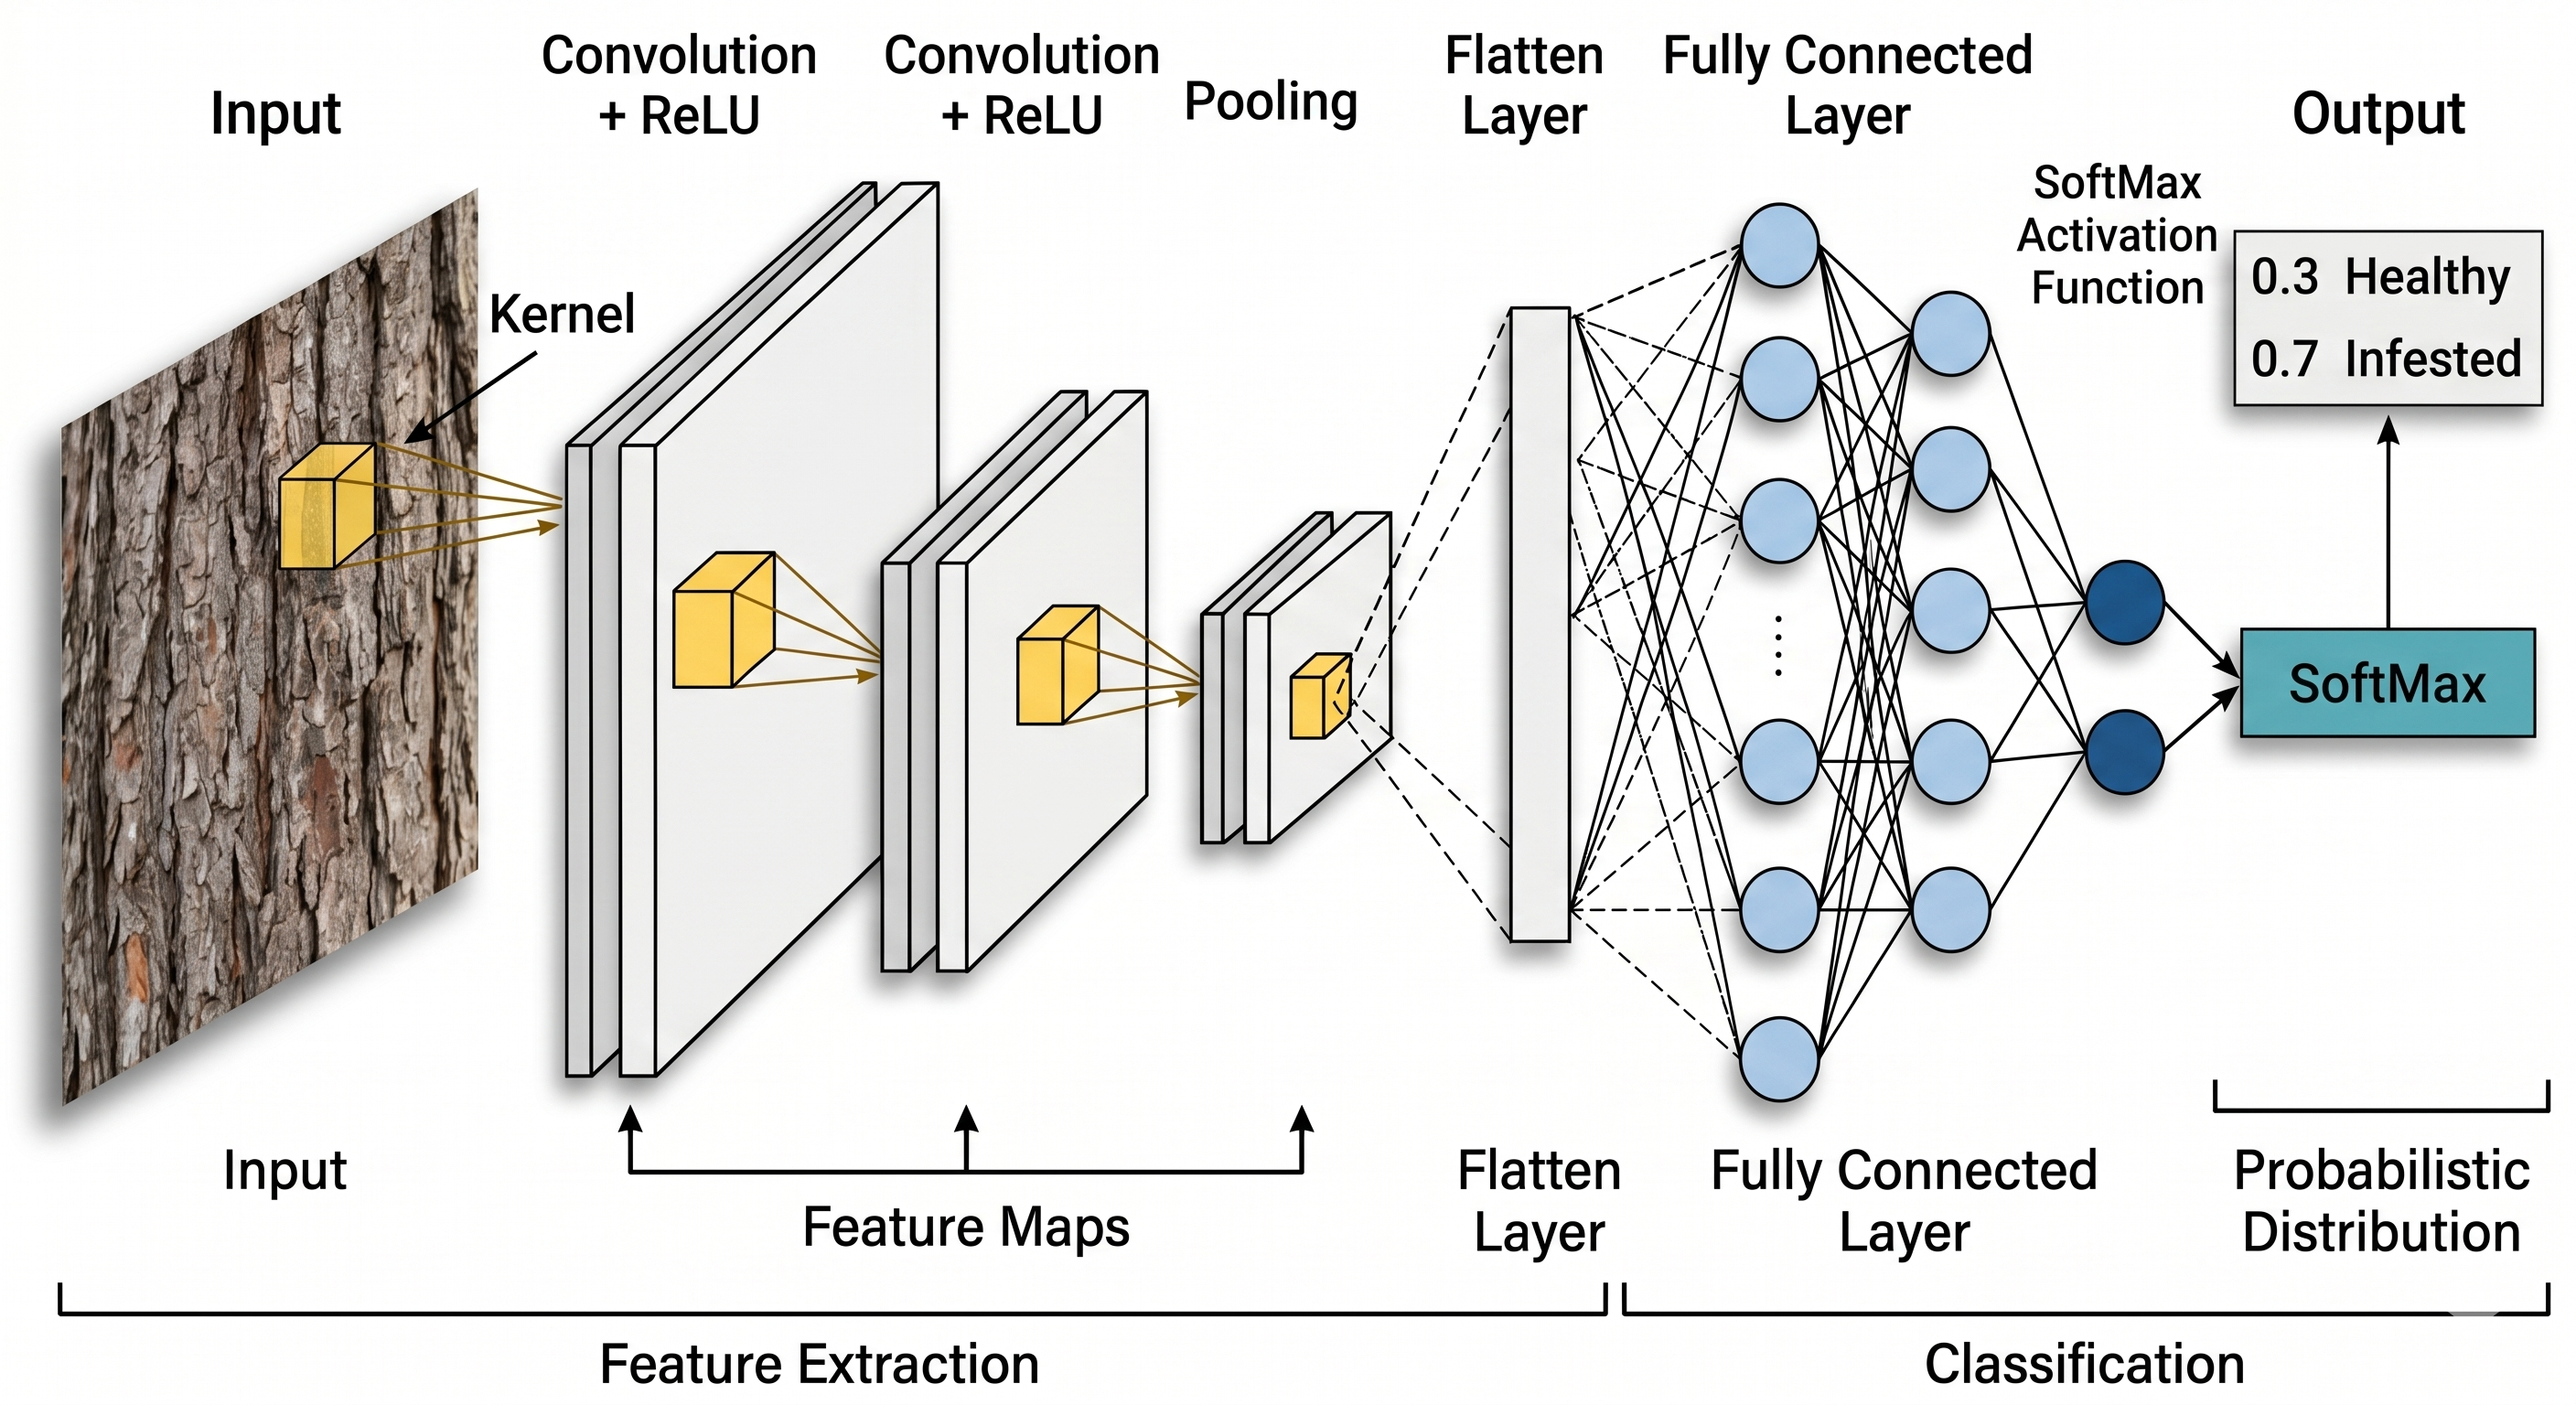
\includegraphics[width=0.9\textwidth]{images/C4/CNNCapas.png}
    \caption{Capas de una CNN}
    
\end{figure}

